% =============================================================================
% STAR ESP32 Firmware Implementation Primer
% Comprehensive Guide for ESP32-S3 Motor Control Firmware
% =============================================================================

\documentclass[11pt,letterpaper]{article}

\usepackage[utf8]{inputenc}
\usepackage[T1]{fontenc}
\usepackage{geometry}
\usepackage{graphicx}
\usepackage{hyperref}
\usepackage{listings}
\usepackage{xcolor}
\usepackage{fancyhdr}
\usepackage{titlesec}
\usepackage{booktabs}
\usepackage{longtable}
\usepackage{tabularx}
\usepackage{enumitem}
\usepackage{amsmath}
\usepackage{tikz}
\usepackage{float}

\usetikzlibrary{shapes.geometric, arrows.meta, positioning, fit, backgrounds}

\geometry{margin=1in}

\hypersetup{
    colorlinks=true,
    linkcolor=blue!70!black,
    urlcolor=cyan!70!black,
    pdftitle={STAR ESP32 Firmware Implementation Primer},
}

\definecolor{codebg}{RGB}{245,245,245}
\definecolor{codeframe}{RGB}{200,200,200}
\definecolor{codekey}{RGB}{0,0,180}
\definecolor{codecomment}{RGB}{0,128,0}
\definecolor{codestring}{RGB}{163,21,21}

\lstset{
    basicstyle=\ttfamily\small,
    backgroundcolor=\color{codebg},
    frame=single,
    rulecolor=\color{codeframe},
    breaklines=true,
    tabsize=2,
    showstringspaces=false,
    numbers=left,
    numberstyle=\tiny\color{gray},
    keywordstyle=\color{codekey}\bfseries,
    commentstyle=\color{codecomment}\itshape,
    stringstyle=\color{codestring},
}

\pagestyle{fancy}
\fancyhf{}
\fancyhead[L]{\leftmark}
\fancyhead[R]{STAR ESP32 Firmware Primer}
\fancyfoot[C]{\thepage}

\title{\textbf{STAR ESP32 Firmware Implementation Primer}\\[0.5cm]
\large ESP32-S3 Motor Control and Sensor Integration Guide}
\author{STAR Development Team}
\date{December 2025}

\begin{document}

\maketitle
\tableofcontents
\newpage

% =============================================================================
\section{Project Overview}
% =============================================================================

\subsection{Purpose}

The \texttt{star-esp32-firmware} project provides real-time motor control, sensor integration, and communication with the Raspberry Pi 5 gateway for the STAR robot platform. It runs on the ESP32-S3 microcontroller using FreeRTOS.

\subsection{Current Implementation Status}

\begin{table}[H]
\centering
\begin{tabular}{|l|c|l|}
\hline
\textbf{Component} & \textbf{Status} & \textbf{Notes} \\
\hline
STAR Framework Core & Complete & DIP architecture, interfaces \\
Bus Abstraction Layer & Complete & I2C, SPI, UART, GPIO, 1-Wire, SMBus \\
Sensor Drivers & Complete & HC-SR04, MPU6050, BNO055, PCA9685, BQ7850 \\
FreeRTOS Tasks & Complete & DHT22, Sensor, LED, Watchdog tasks \\
Error Handling & Complete & Retry logic with exponential backoff \\
Pin Validation & Complete & GPIO conflict detection \\
\hline
Motor Control (MCPWM) & \textbf{TODO} & Center-aligned PWM for 4 motors \\
SPI Peripheral (Pi5 comm) & \textbf{TODO} & Binary protocol for commands \\
TCP Server & \textbf{TODO} & Fallback communication channel \\
PID Controller & \textbf{TODO} & Velocity control loop at 1kHz \\
Encoder Reading & \textbf{TODO} & Quadrature decoder for odometry \\
\hline
\end{tabular}
\caption{Implementation Status Summary}
\end{table}

% =============================================================================
\section{Architecture Overview}
% =============================================================================

\subsection{Dependency Inversion Principle (DIP)}

The firmware follows SOLID principles with emphasis on Dependency Inversion:

\begin{figure}[H]
\centering
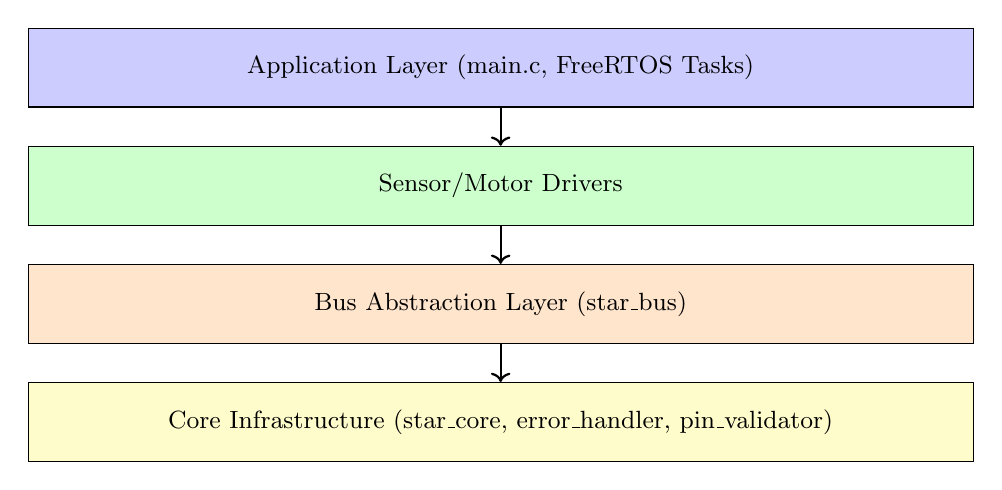
\begin{tikzpicture}[
    layer/.style={draw, rectangle, minimum width=12cm, minimum height=1cm, align=center, font=\small},
    arrow/.style={->, thick}
]
    \node[layer, fill=blue!20] (app) at (0,4) {Application Layer (main.c, FreeRTOS Tasks)};
    \node[layer, fill=green!20] (drivers) at (0,2.5) {Sensor/Motor Drivers};
    \node[layer, fill=orange!20] (bus) at (0,1) {Bus Abstraction Layer (star\_bus)};
    \node[layer, fill=yellow!20] (core) at (0,-0.5) {Core Infrastructure (star\_core, error\_handler, pin\_validator)};

    \draw[arrow] (app) -- (drivers);
    \draw[arrow] (drivers) -- (bus);
    \draw[arrow] (bus) -- (core);
\end{tikzpicture}
\caption{STAR Firmware Layered Architecture}
\end{figure}

\subsection{Directory Structure}

\begin{lstlisting}[language=bash]
star-esp32-firmware/
|-- src/
|   |-- main.c                    # Application entry point
|   |-- system_config.c/h         # Hardware configuration
|   |-- modules/
|   |   |-- shared_data.c/h       # Thread-safe inter-task comm
|   |   +-- led_controller.c/h    # LED control logic
|   +-- tasks/
|       |-- dht22_task.c/h        # Temperature monitoring
|       |-- sensor_task.c/h       # HC-SR04 distance
|       |-- led_task.c/h          # RGB LED feedback
|       +-- watchdog_task.c/h     # System health
|
|-- lib/
|   |-- star_core/                # Abstract interfaces
|   |-- star_error_handler/       # Error handling
|   |-- star_pin_validator/       # GPIO conflict detection
|   |-- star_bus/                 # Unified bus abstraction
|   |-- star_sensor_*/            # Sensor drivers
|   +-- star_bms_bq7850/          # Battery management
|
|-- platformio.ini                # Build configuration
+-- sdkconfig.*                   # ESP-IDF configs
\end{lstlisting}

% =============================================================================
\section{Implementation Tasks}
% =============================================================================

\subsection{Phase 1: Motor Control Implementation}

\subsubsection{Task 1.1: MCPWM Driver}

Create \texttt{lib/star\_motor/} with center-aligned PWM support:

\begin{enumerate}
    \item Create \texttt{star\_motor.h} with motor handle and configuration structs
    \item Implement MCPWM initialization for 4 motors (2 MCPWM units, 2 operators each)
    \item Configure center-aligned (up-down count) mode for reduced EMI
    \item Implement dead-time insertion (prevent H-bridge shoot-through)
    \item Add fault input handling for overcurrent protection
\end{enumerate}

\textbf{Key Parameters:}
\begin{itemize}
    \item PWM Frequency: 20 kHz (above audible range)
    \item Dead Time: 500ns (DRV8243 requirement)
    \item Duty Cycle Resolution: 0.1\%
\end{itemize}

\begin{lstlisting}[language=C, caption=Motor Driver Interface]
typedef struct {
    mcpwm_unit_t unit;
    mcpwm_timer_t timer;
    gpio_num_t pwm_a;
    gpio_num_t pwm_b;
    gpio_num_t fault_pin;
    float max_duty;
} star_motor_config_t;

esp_err_t star_motor_init(star_motor_handle_t* handle,
                          const star_motor_config_t* config,
                          star_error_interface_t* error_iface);
esp_err_t star_motor_set_velocity(star_motor_handle_t* handle,
                                   float velocity_mps);
esp_err_t star_motor_brake(star_motor_handle_t* handle);
esp_err_t star_motor_coast(star_motor_handle_t* handle);
\end{lstlisting}

\subsubsection{Task 1.2: Quadrature Encoder Driver}

Create \texttt{lib/star\_encoder/} for velocity feedback:

\begin{enumerate}
    \item Use ESP32 PCNT (Pulse Counter) peripheral
    \item Configure for quadrature decoding (4x resolution)
    \item Implement velocity calculation from count delta
    \item Add overflow handling for continuous operation
\end{enumerate}

\textbf{Encoder Specifications:}
\begin{itemize}
    \item Resolution: 341.2 counts/revolution
    \item Wheel diameter: 100mm
    \item Distance per count: 0.92mm
\end{itemize}

\subsubsection{Task 1.3: PID Controller}

Create \texttt{lib/star\_pid/} for closed-loop velocity control:

\begin{lstlisting}[language=C, caption=PID Controller Interface]
typedef struct {
    float kp, ki, kd;           // Gains
    float integral_limit;        // Anti-windup
    float output_limit;          // Max PWM duty
    float deadband;              // Ignore small errors
} star_pid_config_t;

void star_pid_init(star_pid_t* pid, const star_pid_config_t* config);
float star_pid_update(star_pid_t* pid, float setpoint, float measurement,
                      float dt);
void star_pid_reset(star_pid_t* pid);
\end{lstlisting}

\textbf{Initial Tuning Values (adjust experimentally):}
\begin{itemize}
    \item $K_p = 1.0$, $K_i = 0.5$, $K_d = 0.1$
    \item Loop rate: 1000 Hz
    \item Integral limit: $\pm$100
\end{itemize}

\subsection{Phase 2: Communication Implementation}

\subsubsection{Task 2.1: SPI Peripheral Driver}

Implement SPI peripheral mode for Pi5 communication:

\begin{enumerate}
    \item Configure ESP32 as SPI peripheral on SPI2 (HSPI)
    \item Implement binary command protocol
    \item Add DMA for efficient transfers
    \item Handle command parsing in ISR-safe manner
\end{enumerate}

\textbf{SPI Pin Mapping:}
\begin{table}[H]
\centering
\begin{tabular}{|l|l|l|}
\hline
\textbf{Signal} & \textbf{Pi5 GPIO} & \textbf{ESP32 GPIO} \\
\hline
COPI & GPIO11 & GPIO13 \\
CIPO & GPIO9 & GPIO12 \\
SCLK & GPIO11 & GPIO14 \\
CS & GPIO8 & GPIO15 \\
\hline
\end{tabular}
\end{table}

\textbf{Command Protocol:}
\begin{lstlisting}[language=C, caption=SPI Command Protocol]
// Command byte definitions
#define CMD_SET_VELOCITY    0x01  // Set wheel velocities
#define CMD_EMERGENCY_STOP  0x02  // Immediate stop
#define CMD_GET_ENCODERS    0x03  // Read encoder counts
#define CMD_SET_MOTOR       0x04  // Direct motor control
#define CMD_PING            0x05  // Connection test
#define CMD_GET_TELEMETRY   0x06  // Battery, temp, status

// Packet format: [CMD (1)] [LENGTH (1)] [DATA (N)] [CRC8 (1)]
typedef struct __attribute__((packed)) {
    uint8_t command;
    uint8_t length;
    uint8_t data[32];
    uint8_t crc8;
} spi_packet_t;

// Velocity command payload
typedef struct __attribute__((packed)) {
    float left_velocity;   // m/s
    float right_velocity;  // m/s
    uint32_t timestamp;    // ms since boot
} velocity_cmd_t;
\end{lstlisting}

\subsubsection{Task 2.2: TCP Server (Fallback)}

Implement TCP server as backup communication channel:

\begin{enumerate}
    \item Create TCP server on port 5000
    \item Accept JSON-formatted commands
    \item Integrate with WiFi station mode (connect to Pi5 AP)
    \item Implement connection timeout and reconnection
\end{enumerate}

\begin{lstlisting}[language=C, caption=TCP Command Format (JSON)]
// Velocity command
{"command": "velocity", "params": {"left": 0.5, "right": 0.5}}

// Emergency stop
{"command": "emergency_stop"}

// Response format
{"success": true, "message": "OK", "data": {...}}
\end{lstlisting}

\subsection{Phase 3: Integration}

\subsubsection{Task 3.1: Motor Control Task}

Create \texttt{src/tasks/motor\_task.c}:

\begin{enumerate}
    \item Run PID loop at 1000 Hz (1ms period)
    \item Read encoder velocity feedback
    \item Compute PID output and apply to MCPWM
    \item Publish odometry to shared data
    \item Handle emergency stop interrupt
\end{enumerate}

\begin{lstlisting}[language=C, caption=Motor Control Task Structure]
void motor_control_task(void* pvParameters) {
    TickType_t last_wake = xTaskGetTickCount();
    const TickType_t period = pdMS_TO_TICKS(1);  // 1kHz

    while (1) {
        // 1. Read velocity setpoints from queue
        velocity_cmd_t cmd;
        if (xQueuePeek(velocity_queue, &cmd, 0) == pdTRUE) {
            target_left = cmd.left_velocity;
            target_right = cmd.right_velocity;
        }

        // 2. Read encoder velocities
        float vel_left = star_encoder_get_velocity(&enc_left);
        float vel_right = star_encoder_get_velocity(&enc_right);

        // 3. Update PID controllers
        float duty_left = star_pid_update(&pid_left, target_left,
                                          vel_left, 0.001f);
        float duty_right = star_pid_update(&pid_right, target_right,
                                           vel_right, 0.001f);

        // 4. Apply to motors
        star_motor_set_duty(&motor_left, duty_left);
        star_motor_set_duty(&motor_right, duty_right);

        // 5. Update odometry
        update_odometry(vel_left, vel_right, 0.001f);

        vTaskDelayUntil(&last_wake, period);
    }
}
\end{lstlisting}

\subsubsection{Task 3.2: Communication Task}

Create \texttt{src/tasks/comm\_task.c}:

\begin{enumerate}
    \item Poll SPI peripheral for incoming commands
    \item Parse and validate packets
    \item Dispatch to appropriate handlers
    \item Send responses/telemetry
    \item Fallback to TCP if SPI fails
\end{enumerate}

% =============================================================================
\section{Testing Plan}
% =============================================================================

\subsection{Unit Tests}

\begin{enumerate}
    \item \textbf{PID Controller}: Test with simulated plant, verify convergence
    \item \textbf{Encoder Driver}: Test count accuracy, overflow handling
    \item \textbf{Motor Driver}: Test PWM generation, dead-time
    \item \textbf{SPI Protocol}: Test packet parsing, CRC validation
\end{enumerate}

\subsection{Integration Tests}

\begin{enumerate}
    \item \textbf{Motor + Encoder}: Closed-loop step response test
    \item \textbf{SPI + Motor}: Command-to-motion latency measurement
    \item \textbf{Full System}: Velocity tracking accuracy at various speeds
\end{enumerate}

\subsection{Acceptance Criteria}

\begin{table}[H]
\centering
\begin{tabular}{|l|l|}
\hline
\textbf{Metric} & \textbf{Target} \\
\hline
PID loop rate & 1000 Hz $\pm$ 1\% \\
Velocity tracking error & $<$ 5\% at steady state \\
Command latency (SPI) & $<$ 1ms \\
Emergency stop time & $<$ 10ms \\
\hline
\end{tabular}
\end{table}

% =============================================================================
\section{Build and Flash Instructions}
% =============================================================================

\subsection{Prerequisites}

\begin{lstlisting}[language=bash]
# Install PlatformIO
pip install platformio

# Install ESP-IDF (handled by PlatformIO)
pio pkg install
\end{lstlisting}

\subsection{Build Commands}

\begin{lstlisting}[language=bash]
# Build for ESP32-S3
pio run -e esp32s3

# Build for ESP32-WROOM (dev board)
pio run -e esp32_wroom

# Upload firmware
pio run -e esp32s3 --target upload

# Monitor serial output
pio device monitor -b 115200
\end{lstlisting}

\subsection{Configuration}

Edit \texttt{sdkconfig.esp32s3} for production settings:
\begin{itemize}
    \item Enable brownout detection
    \item Set CPU frequency to 240 MHz
    \item Configure flash size (16 MB)
    \item Enable PSRAM if needed
\end{itemize}

% =============================================================================
\section{References}
% =============================================================================

\begin{itemize}
    \item ESP-IDF MCPWM Documentation: \url{https://docs.espressif.com/projects/esp-idf/en/latest/esp32s3/api-reference/peripherals/mcpwm.html}
    \item ESP-IDF SPI Peripheral: \url{https://docs.espressif.com/projects/esp-idf/en/latest/esp32s3/api-reference/peripherals/spi_slave.html}
    \item FreeRTOS Task Notifications: \url{https://www.freertos.org/RTOS-task-notifications.html}
    \item DRV8243 Datasheet: TI SLVSFN4
    \item STAR FTP Section 16: Embedded Implementation
    \item STAR Software Architecture Primer: Section 12 (ESP32 Firmware)
\end{itemize}

\end{document}
